% Generated by ArticleSignalDiagrams. Opaque vector fills only.
\documentclass[10pt,tikz,border=5pt]{standalone}
\usepackage{lmodern}
\usetikzlibrary{fit}
\begin{document}
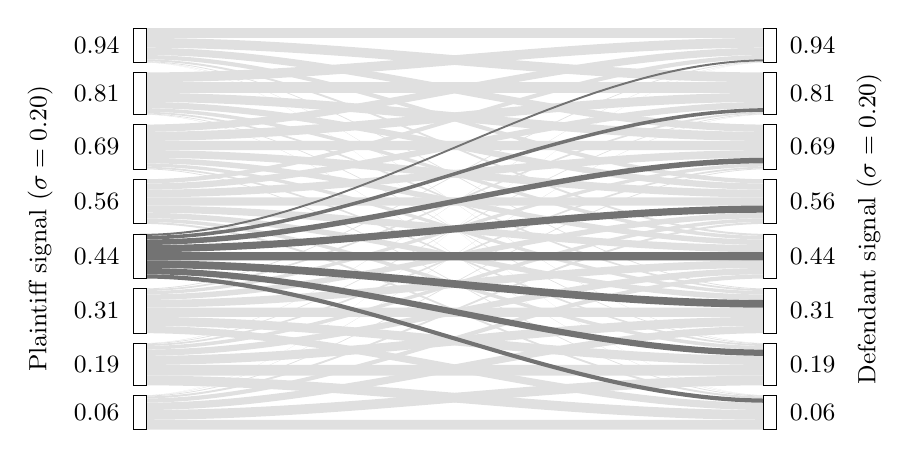
\begin{tikzpicture}[x=1cm,y=1cm,font=\small]\path[fill=black!12,draw=none] (3.3,-5.1) .. controls (6,-5.1) and (8.6,-5.1) .. (11.3,-5.1) -- (11.3,-4.974717) .. controls (8.6,-4.974717) and (6,-4.974717) .. (3.3,-4.974717) -- cycle;
\path[fill=black!12,draw=none] (3.3,-4.974717) .. controls (6,-4.974717) and (8.6,-4.536357) .. (11.3,-4.536357) -- (11.3,-4.41275) .. controls (8.6,-4.41275) and (6,-4.85111) .. (3.3,-4.85111) -- cycle;
\path[fill=black!12,draw=none] (3.3,-4.85111) .. controls (6,-4.85111) and (8.6,-3.874105) .. (11.3,-3.874105) -- (11.3,-3.781808) .. controls (8.6,-3.781808) and (6,-4.758813) .. (3.3,-4.758813) -- cycle;
\path[fill=black!12,draw=none] (3.3,-4.758813) .. controls (6,-4.758813) and (8.6,-3.179626) .. (11.3,-3.179626) -- (11.3,-3.12571) .. controls (8.6,-3.12571) and (6,-4.704897) .. (3.3,-4.704897) -- cycle;
\path[fill=black!12,draw=none] (3.3,-4.704897) .. controls (6,-4.704897) and (8.6,-2.485714) .. (11.3,-2.485714) -- (11.3,-2.460191) .. controls (8.6,-2.460191) and (6,-4.679374) .. (3.3,-4.679374) -- cycle;
\path[fill=black!12,draw=none] (3.3,-4.679374) .. controls (6,-4.679374) and (8.6,-1.791803) .. (11.3,-1.791803) -- (11.3,-1.781717) .. controls (8.6,-1.781717) and (6,-4.669288) .. (3.3,-4.669288) -- cycle;
\path[fill=black!12,draw=none] (3.3,-4.669288) .. controls (6,-4.669288) and (8.6,-1.097324) .. (11.3,-1.097324) -- (11.3,-1.093937) .. controls (8.6,-1.093937) and (6,-4.665901) .. (3.3,-4.665901) -- cycle;
\path[fill=black!12,draw=none] (3.3,-4.665901) .. controls (6,-4.665901) and (8.6,-0.435071) .. (11.3,-0.435071) -- (11.3,-0.434099) .. controls (8.6,-0.434099) and (6,-4.664929) .. (3.3,-4.664929) -- cycle;
\path[fill=black!12,draw=none] (3.3,-4.536357) .. controls (6,-4.536357) and (8.6,-4.974717) .. (11.3,-4.974717) -- (11.3,-4.85111) .. controls (8.6,-4.85111) and (6,-4.41275) .. (3.3,-4.41275) -- cycle;
\path[fill=black!12,draw=none] (3.3,-4.41275) .. controls (6,-4.41275) and (8.6,-4.41275) .. (11.3,-4.41275) -- (11.3,-4.278032) .. controls (8.6,-4.278032) and (6,-4.278032) .. (3.3,-4.278032) -- cycle;
\path[fill=black!12,draw=none] (3.3,-4.278032) .. controls (6,-4.278032) and (8.6,-3.781808) .. (11.3,-3.781808) -- (11.3,-3.666931) .. controls (8.6,-3.666931) and (6,-4.163155) .. (3.3,-4.163155) -- cycle;
\path[fill=black!12,draw=none] (3.3,-4.163155) .. controls (6,-4.163155) and (8.6,-3.12571) .. (11.3,-3.12571) -- (11.3,-3.046315) .. controls (8.6,-3.046315) and (6,-4.08376) .. (3.3,-4.08376) -- cycle;
\path[fill=black!12,draw=none] (3.3,-4.08376) .. controls (6,-4.08376) and (8.6,-2.460191) .. (11.3,-2.460191) -- (11.3,-2.414381) .. controls (8.6,-2.414381) and (6,-4.03795) .. (3.3,-4.03795) -- cycle;
\path[fill=black!12,draw=none] (3.3,-4.03795) .. controls (6,-4.03795) and (8.6,-1.781717) .. (11.3,-1.781717) -- (11.3,-1.759254) .. controls (8.6,-1.759254) and (6,-4.015487) .. (3.3,-4.015487) -- cycle;
\path[fill=black!12,draw=none] (3.3,-4.015487) .. controls (6,-4.015487) and (8.6,-1.093937) .. (11.3,-1.093937) -- (11.3,-1.084513) .. controls (8.6,-1.084513) and (6,-4.006063) .. (3.3,-4.006063) -- cycle;
\path[fill=black!12,draw=none] (3.3,-4.006063) .. controls (6,-4.006063) and (8.6,-0.434099) .. (11.3,-0.434099) -- (11.3,-0.430712) .. controls (8.6,-0.430712) and (6,-4.002676) .. (3.3,-4.002676) -- cycle;
\path[fill=black!12,draw=none] (3.3,-3.874105) .. controls (6,-3.874105) and (8.6,-4.85111) .. (11.3,-4.85111) -- (11.3,-4.758813) .. controls (8.6,-4.758813) and (6,-3.781808) .. (3.3,-3.781808) -- cycle;
\path[fill=black!12,draw=none] (3.3,-3.781808) .. controls (6,-3.781808) and (8.6,-4.278032) .. (11.3,-4.278032) -- (11.3,-4.163155) .. controls (8.6,-4.163155) and (6,-3.666931) .. (3.3,-3.666931) -- cycle;
\path[fill=black!12,draw=none] (3.3,-3.666931) .. controls (6,-3.666931) and (8.6,-3.666931) .. (11.3,-3.666931) -- (11.3,-3.551039) .. controls (8.6,-3.551039) and (6,-3.551039) .. (3.3,-3.551039) -- cycle;
\path[fill=black!12,draw=none] (3.3,-3.551039) .. controls (6,-3.551039) and (8.6,-3.046315) .. (11.3,-3.046315) -- (11.3,-2.948703) .. controls (8.6,-2.948703) and (6,-3.453427) .. (3.3,-3.453427) -- cycle;
\path[fill=black!12,draw=none] (3.3,-3.453427) .. controls (6,-3.453427) and (8.6,-2.414381) .. (11.3,-2.414381) -- (11.3,-2.344504) .. controls (8.6,-2.344504) and (6,-3.38355) .. (3.3,-3.38355) -- cycle;
\path[fill=black!12,draw=none] (3.3,-3.38355) .. controls (6,-3.38355) and (8.6,-1.759254) .. (11.3,-1.759254) -- (11.3,-1.71645) .. controls (8.6,-1.71645) and (6,-3.340746) .. (3.3,-3.340746) -- cycle;
\path[fill=black!12,draw=none] (3.3,-3.340746) .. controls (6,-3.340746) and (8.6,-1.084513) .. (11.3,-1.084513) -- (11.3,-1.06205) .. controls (8.6,-1.06205) and (6,-3.318283) .. (3.3,-3.318283) -- cycle;
\path[fill=black!12,draw=none] (3.3,-3.318283) .. controls (6,-3.318283) and (8.6,-0.430712) .. (11.3,-0.430712) -- (11.3,-0.420626) .. controls (8.6,-0.420626) and (6,-3.308197) .. (3.3,-3.308197) -- cycle;
\path[fill=black!12,draw=none] (3.3,-2.485714) .. controls (6,-2.485714) and (8.6,-4.704897) .. (11.3,-4.704897) -- (11.3,-4.679374) .. controls (8.6,-4.679374) and (6,-2.460191) .. (3.3,-2.460191) -- cycle;
\path[fill=black!12,draw=none] (3.3,-2.460191) .. controls (6,-2.460191) and (8.6,-4.08376) .. (11.3,-4.08376) -- (11.3,-4.03795) .. controls (8.6,-4.03795) and (6,-2.414381) .. (3.3,-2.414381) -- cycle;
\path[fill=black!12,draw=none] (3.3,-2.414381) .. controls (6,-2.414381) and (8.6,-3.453427) .. (11.3,-3.453427) -- (11.3,-3.38355) .. controls (8.6,-3.38355) and (6,-2.344504) .. (3.3,-2.344504) -- cycle;
\path[fill=black!12,draw=none] (3.3,-2.344504) .. controls (6,-2.344504) and (8.6,-2.846703) .. (11.3,-2.846703) -- (11.3,-2.755496) .. controls (8.6,-2.755496) and (6,-2.253297) .. (3.3,-2.253297) -- cycle;
\path[fill=black!12,draw=none] (3.3,-2.253297) .. controls (6,-2.253297) and (8.6,-2.253297) .. (11.3,-2.253297) -- (11.3,-2.151297) .. controls (8.6,-2.151297) and (6,-2.151297) .. (3.3,-2.151297) -- cycle;
\path[fill=black!12,draw=none] (3.3,-2.151297) .. controls (6,-2.151297) and (8.6,-1.646573) .. (11.3,-1.646573) -- (11.3,-1.548961) .. controls (8.6,-1.548961) and (6,-2.053685) .. (3.3,-2.053685) -- cycle;
\path[fill=black!12,draw=none] (3.3,-2.053685) .. controls (6,-2.053685) and (8.6,-1.01624) .. (11.3,-1.01624) -- (11.3,-0.936845) .. controls (8.6,-0.936845) and (6,-1.97429) .. (3.3,-1.97429) -- cycle;
\path[fill=black!12,draw=none] (3.3,-1.97429) .. controls (6,-1.97429) and (8.6,-0.395103) .. (11.3,-0.395103) -- (11.3,-0.341187) .. controls (8.6,-0.341187) and (6,-1.920374) .. (3.3,-1.920374) -- cycle;
\path[fill=black!12,draw=none] (3.3,-1.791803) .. controls (6,-1.791803) and (8.6,-4.679374) .. (11.3,-4.679374) -- (11.3,-4.669288) .. controls (8.6,-4.669288) and (6,-1.781717) .. (3.3,-1.781717) -- cycle;
\path[fill=black!12,draw=none] (3.3,-1.781717) .. controls (6,-1.781717) and (8.6,-4.03795) .. (11.3,-4.03795) -- (11.3,-4.015487) .. controls (8.6,-4.015487) and (6,-1.759254) .. (3.3,-1.759254) -- cycle;
\path[fill=black!12,draw=none] (3.3,-1.759254) .. controls (6,-1.759254) and (8.6,-3.38355) .. (11.3,-3.38355) -- (11.3,-3.340746) .. controls (8.6,-3.340746) and (6,-1.71645) .. (3.3,-1.71645) -- cycle;
\path[fill=black!12,draw=none] (3.3,-1.71645) .. controls (6,-1.71645) and (8.6,-2.755496) .. (11.3,-2.755496) -- (11.3,-2.685619) .. controls (8.6,-2.685619) and (6,-1.646573) .. (3.3,-1.646573) -- cycle;
\path[fill=black!12,draw=none] (3.3,-1.646573) .. controls (6,-1.646573) and (8.6,-2.151297) .. (11.3,-2.151297) -- (11.3,-2.053685) .. controls (8.6,-2.053685) and (6,-1.548961) .. (3.3,-1.548961) -- cycle;
\path[fill=black!12,draw=none] (3.3,-1.548961) .. controls (6,-1.548961) and (8.6,-1.548961) .. (11.3,-1.548961) -- (11.3,-1.433069) .. controls (8.6,-1.433069) and (6,-1.433069) .. (3.3,-1.433069) -- cycle;
\path[fill=black!12,draw=none] (3.3,-1.433069) .. controls (6,-1.433069) and (8.6,-0.936845) .. (11.3,-0.936845) -- (11.3,-0.821968) .. controls (8.6,-0.821968) and (6,-1.318192) .. (3.3,-1.318192) -- cycle;
\path[fill=black!12,draw=none] (3.3,-1.318192) .. controls (6,-1.318192) and (8.6,-0.341187) .. (11.3,-0.341187) -- (11.3,-0.24889) .. controls (8.6,-0.24889) and (6,-1.225895) .. (3.3,-1.225895) -- cycle;
\path[fill=black!12,draw=none] (3.3,-1.097324) .. controls (6,-1.097324) and (8.6,-4.669288) .. (11.3,-4.669288) -- (11.3,-4.665901) .. controls (8.6,-4.665901) and (6,-1.093937) .. (3.3,-1.093937) -- cycle;
\path[fill=black!12,draw=none] (3.3,-1.093937) .. controls (6,-1.093937) and (8.6,-4.015487) .. (11.3,-4.015487) -- (11.3,-4.006063) .. controls (8.6,-4.006063) and (6,-1.084513) .. (3.3,-1.084513) -- cycle;
\path[fill=black!12,draw=none] (3.3,-1.084513) .. controls (6,-1.084513) and (8.6,-3.340746) .. (11.3,-3.340746) -- (11.3,-3.318283) .. controls (8.6,-3.318283) and (6,-1.06205) .. (3.3,-1.06205) -- cycle;
\path[fill=black!12,draw=none] (3.3,-1.06205) .. controls (6,-1.06205) and (8.6,-2.685619) .. (11.3,-2.685619) -- (11.3,-2.639809) .. controls (8.6,-2.639809) and (6,-1.01624) .. (3.3,-1.01624) -- cycle;
\path[fill=black!12,draw=none] (3.3,-1.01624) .. controls (6,-1.01624) and (8.6,-2.053685) .. (11.3,-2.053685) -- (11.3,-1.97429) .. controls (8.6,-1.97429) and (6,-0.936845) .. (3.3,-0.936845) -- cycle;
\path[fill=black!12,draw=none] (3.3,-0.936845) .. controls (6,-0.936845) and (8.6,-1.433069) .. (11.3,-1.433069) -- (11.3,-1.318192) .. controls (8.6,-1.318192) and (6,-0.821968) .. (3.3,-0.821968) -- cycle;
\path[fill=black!12,draw=none] (3.3,-0.821968) .. controls (6,-0.821968) and (8.6,-0.821968) .. (11.3,-0.821968) -- (11.3,-0.68725) .. controls (8.6,-0.68725) and (6,-0.68725) .. (3.3,-0.68725) -- cycle;
\path[fill=black!12,draw=none] (3.3,-0.68725) .. controls (6,-0.68725) and (8.6,-0.24889) .. (11.3,-0.24889) -- (11.3,-0.125283) .. controls (8.6,-0.125283) and (6,-0.563643) .. (3.3,-0.563643) -- cycle;
\path[fill=black!12,draw=none] (3.3,-0.435071) .. controls (6,-0.435071) and (8.6,-4.665901) .. (11.3,-4.665901) -- (11.3,-4.664929) .. controls (8.6,-4.664929) and (6,-0.434099) .. (3.3,-0.434099) -- cycle;
\path[fill=black!12,draw=none] (3.3,-0.434099) .. controls (6,-0.434099) and (8.6,-4.006063) .. (11.3,-4.006063) -- (11.3,-4.002676) .. controls (8.6,-4.002676) and (6,-0.430712) .. (3.3,-0.430712) -- cycle;
\path[fill=black!12,draw=none] (3.3,-0.430712) .. controls (6,-0.430712) and (8.6,-3.318283) .. (11.3,-3.318283) -- (11.3,-3.308197) .. controls (8.6,-3.308197) and (6,-0.420626) .. (3.3,-0.420626) -- cycle;
\path[fill=black!12,draw=none] (3.3,-0.420626) .. controls (6,-0.420626) and (8.6,-2.639809) .. (11.3,-2.639809) -- (11.3,-2.614286) .. controls (8.6,-2.614286) and (6,-0.395103) .. (3.3,-0.395103) -- cycle;
\path[fill=black!12,draw=none] (3.3,-0.395103) .. controls (6,-0.395103) and (8.6,-1.97429) .. (11.3,-1.97429) -- (11.3,-1.920374) .. controls (8.6,-1.920374) and (6,-0.341187) .. (3.3,-0.341187) -- cycle;
\path[fill=black!12,draw=none] (3.3,-0.341187) .. controls (6,-0.341187) and (8.6,-1.318192) .. (11.3,-1.318192) -- (11.3,-1.225895) .. controls (8.6,-1.225895) and (6,-0.24889) .. (3.3,-0.24889) -- cycle;
\path[fill=black!12,draw=none] (3.3,-0.24889) .. controls (6,-0.24889) and (8.6,-0.68725) .. (11.3,-0.68725) -- (11.3,-0.563643) .. controls (8.6,-0.563643) and (6,-0.125283) .. (3.3,-0.125283) -- cycle;
\path[fill=black!12,draw=none] (3.3,-0.125283) .. controls (6,-0.125283) and (8.6,-0.125283) .. (11.3,-0.125283) -- (11.3,0) .. controls (8.6,0) and (6,0) .. (3.3,0) -- cycle;
\path[fill=black!55,draw=none] (3.3,-3.179626) .. controls (6,-3.179626) and (8.6,-4.758813) .. (11.3,-4.758813) -- (11.3,-4.704897) .. controls (8.6,-4.704897) and (6,-3.12571) .. (3.3,-3.12571) -- cycle;
\path[fill=black!55,draw=none] (3.3,-3.12571) .. controls (6,-3.12571) and (8.6,-4.163155) .. (11.3,-4.163155) -- (11.3,-4.08376) .. controls (8.6,-4.08376) and (6,-3.046315) .. (3.3,-3.046315) -- cycle;
\path[fill=black!55,draw=none] (3.3,-3.046315) .. controls (6,-3.046315) and (8.6,-3.551039) .. (11.3,-3.551039) -- (11.3,-3.453427) .. controls (8.6,-3.453427) and (6,-2.948703) .. (3.3,-2.948703) -- cycle;
\path[fill=black!55,draw=none] (3.3,-2.948703) .. controls (6,-2.948703) and (8.6,-2.948703) .. (11.3,-2.948703) -- (11.3,-2.846703) .. controls (8.6,-2.846703) and (6,-2.846703) .. (3.3,-2.846703) -- cycle;
\path[fill=black!55,draw=none] (3.3,-2.846703) .. controls (6,-2.846703) and (8.6,-2.344504) .. (11.3,-2.344504) -- (11.3,-2.253297) .. controls (8.6,-2.253297) and (6,-2.755496) .. (3.3,-2.755496) -- cycle;
\path[fill=black!55,draw=none] (3.3,-2.755496) .. controls (6,-2.755496) and (8.6,-1.71645) .. (11.3,-1.71645) -- (11.3,-1.646573) .. controls (8.6,-1.646573) and (6,-2.685619) .. (3.3,-2.685619) -- cycle;
\path[fill=black!55,draw=none] (3.3,-2.685619) .. controls (6,-2.685619) and (8.6,-1.06205) .. (11.3,-1.06205) -- (11.3,-1.01624) .. controls (8.6,-1.01624) and (6,-2.639809) .. (3.3,-2.639809) -- cycle;
\path[fill=black!55,draw=none] (3.3,-2.639809) .. controls (6,-2.639809) and (8.6,-0.420626) .. (11.3,-0.420626) -- (11.3,-0.395103) .. controls (8.6,-0.395103) and (6,-2.614286) .. (3.3,-2.614286) -- cycle;
\coordinate (axis-midline-0) at (0,-2.55);
\path[fill=white,draw=black,line width=0.3pt] (3.22,-5.1) rectangle (3.38,-4.664929);
\node[anchor=east,fill=white,inner sep=2pt] (bucket-0-0-0) at (3.12,-4.882464) {0.06};
\path[fill=white,draw=black,line width=0.3pt] (3.22,-4.536357) rectangle (3.38,-4.002676);
\node[anchor=east,fill=white,inner sep=2pt] (bucket-0-0-1) at (3.12,-4.269517) {0.19};
\path[fill=white,draw=black,line width=0.3pt] (3.22,-3.874105) rectangle (3.38,-3.308197);
\node[anchor=east,fill=white,inner sep=2pt] (bucket-0-0-2) at (3.12,-3.591151) {0.31};
\path[fill=white,draw=black,line width=0.3pt] (3.22,-3.179626) rectangle (3.38,-2.614286);
\node[anchor=east,fill=white,inner sep=2pt] (bucket-0-0-3) at (3.12,-2.896956) {0.44};
\path[fill=white,draw=black,line width=0.3pt] (3.22,-2.485714) rectangle (3.38,-1.920374);
\node[anchor=east,fill=white,inner sep=2pt] (bucket-0-0-4) at (3.12,-2.203044) {0.56};
\path[fill=white,draw=black,line width=0.3pt] (3.22,-1.791803) rectangle (3.38,-1.225895);
\node[anchor=east,fill=white,inner sep=2pt] (bucket-0-0-5) at (3.12,-1.508849) {0.69};
\path[fill=white,draw=black,line width=0.3pt] (3.22,-1.097324) rectangle (3.38,-0.563643);
\node[anchor=east,fill=white,inner sep=2pt] (bucket-0-0-6) at (3.12,-0.830483) {0.81};
\path[fill=white,draw=black,line width=0.3pt] (3.22,-0.435071) rectangle (3.38,0);
\node[anchor=east,fill=white,inner sep=2pt] (bucket-0-0-7) at (3.12,-0.217536) {0.94};
\node[fit=(bucket-0-0-0) (bucket-0-0-1) (bucket-0-0-2) (bucket-0-0-3) (bucket-0-0-4) (bucket-0-0-5) (bucket-0-0-6) (bucket-0-0-7),inner sep=0pt] (source-labels-0) {};
\coordinate (axis-title-0-0) at (source-labels-0.west |- axis-midline-0);
\node[rotate=90,anchor=south,inner sep=0pt] at ([xshift=-0.18cm]axis-title-0-0) {Plaintiff signal ($\sigma=0.20$)};
\path[fill=white,draw=black,line width=0.3pt] (11.22,-5.1) rectangle (11.38,-4.664929);
\node[anchor=west,fill=white,inner sep=2pt] (bucket-0-1-0) at (11.48,-4.882464) {0.06};
\path[fill=white,draw=black,line width=0.3pt] (11.22,-4.536357) rectangle (11.38,-4.002676);
\node[anchor=west,fill=white,inner sep=2pt] (bucket-0-1-1) at (11.48,-4.269517) {0.19};
\path[fill=white,draw=black,line width=0.3pt] (11.22,-3.874105) rectangle (11.38,-3.308197);
\node[anchor=west,fill=white,inner sep=2pt] (bucket-0-1-2) at (11.48,-3.591151) {0.31};
\path[fill=white,draw=black,line width=0.3pt] (11.22,-3.179626) rectangle (11.38,-2.614286);
\node[anchor=west,fill=white,inner sep=2pt] (bucket-0-1-3) at (11.48,-2.896956) {0.44};
\path[fill=white,draw=black,line width=0.3pt] (11.22,-2.485714) rectangle (11.38,-1.920374);
\node[anchor=west,fill=white,inner sep=2pt] (bucket-0-1-4) at (11.48,-2.203044) {0.56};
\path[fill=white,draw=black,line width=0.3pt] (11.22,-1.791803) rectangle (11.38,-1.225895);
\node[anchor=west,fill=white,inner sep=2pt] (bucket-0-1-5) at (11.48,-1.508849) {0.69};
\path[fill=white,draw=black,line width=0.3pt] (11.22,-1.097324) rectangle (11.38,-0.563643);
\node[anchor=west,fill=white,inner sep=2pt] (bucket-0-1-6) at (11.48,-0.830483) {0.81};
\path[fill=white,draw=black,line width=0.3pt] (11.22,-0.435071) rectangle (11.38,0);
\node[anchor=west,fill=white,inner sep=2pt] (bucket-0-1-7) at (11.48,-0.217536) {0.94};
\node[fit=(bucket-0-1-0) (bucket-0-1-1) (bucket-0-1-2) (bucket-0-1-3) (bucket-0-1-4) (bucket-0-1-5) (bucket-0-1-6) (bucket-0-1-7),inner sep=0pt] (destination-labels-0) {};
\coordinate (axis-title-0-1) at (destination-labels-0.east |- axis-midline-0);
\node[rotate=90,anchor=north,inner sep=0pt] at ([xshift=0.18cm]axis-title-0-1) {Defendant signal ($\sigma=0.20$)};
\end{tikzpicture}
\end{document}

